\section{Resultados}
Para guiar toda la parte de resultados, se realizo una interfaz grafica con el uso de la librería
\textbf{CustomTkinter} que permite crear una aplicación completamente funcional de escritorio para 
que el usuario pueda interactuar con la red neuronal LeNet 5. La aplicación permite al usuario
las siguientes funcionaliades:

\begin{itemize}
    \item \textbf{Ver Datos de Entrenamiento:} El usuario puede visualizar los datos de entrenamiento, 
    esta funcionalidad muestra 5 imagenes de ejemplo por cada clase de la base de datos.

    \begin{figure}[htbp]
        \centering
        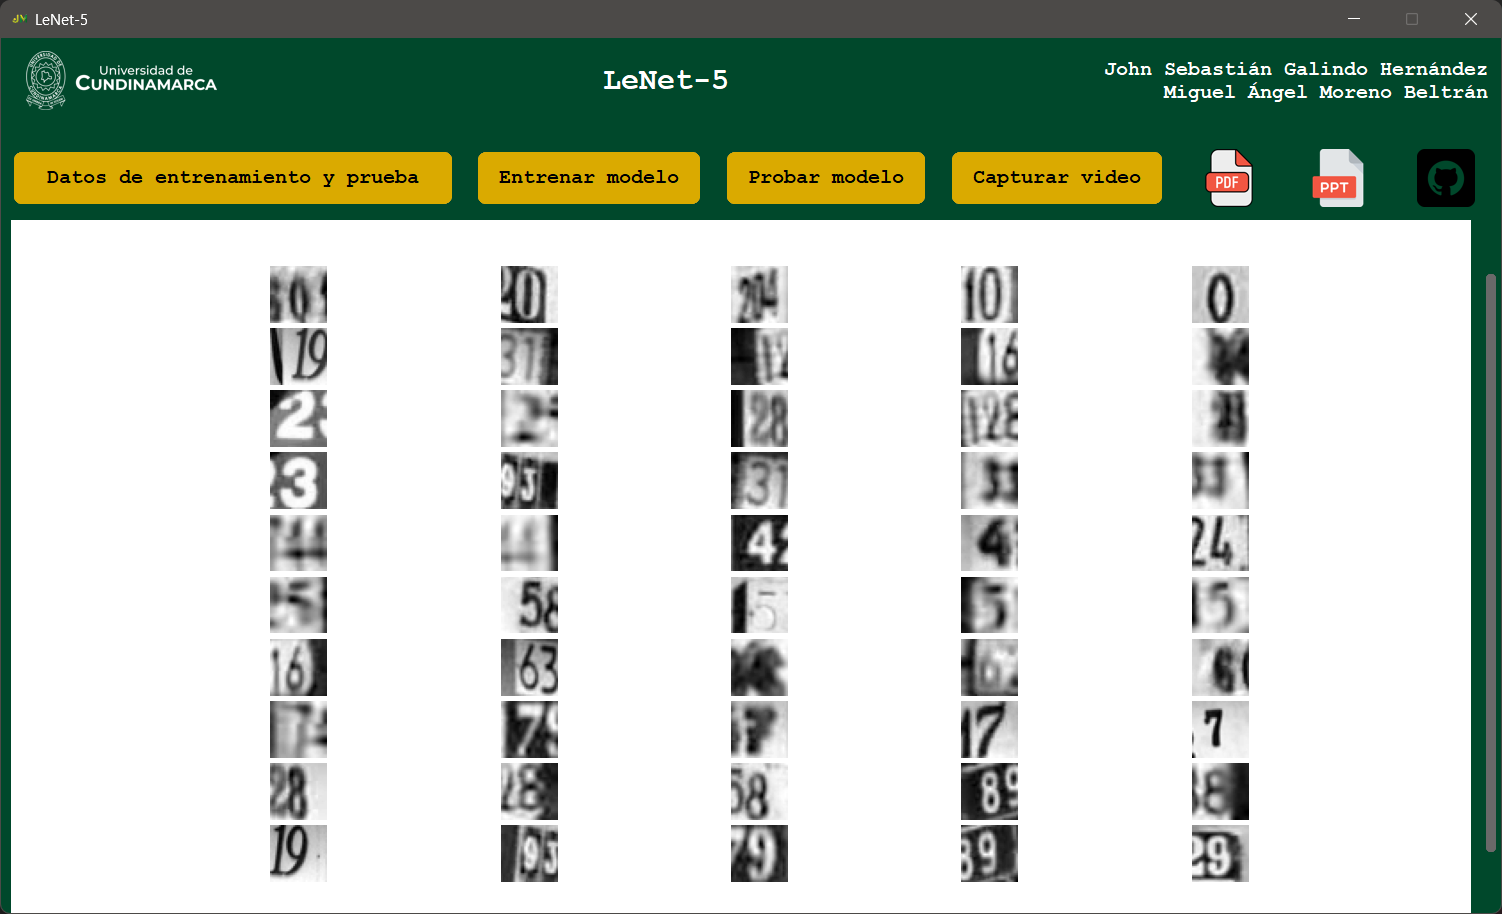
\includegraphics[width=\linewidth]{src/figures/info_function.png}
        \caption{Datos de Entrenamiento}
        \label{fig:TrainingData}
    \end{figure}

    \item \textbf{Entrenar la Red:} El usuario puede entrenar la red neuronal LeNet 5 con los datos de
    MNIST o SVHN, después de que el usuario seleccione la base de datos, la red carga los datos y 
    comienza el entrenamiento, el entrenamiento se puede ver por consola y la arquitectura de la red
    junto con los pesos resultantes para los kernels de la primera y segunda capa convolucional.

    \begin{figure}[htbp]
        \centering
        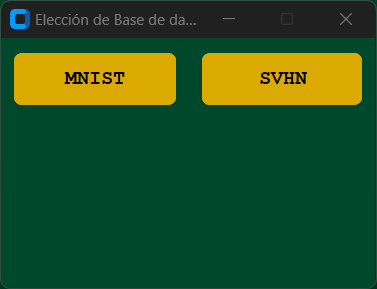
\includegraphics[width=0.6\linewidth]{src/figures/eleccion_bd.png}
        \caption{Selección de la Base de Datos} 
        \label{fig:bd_selection} 
    \end{figure}

    \begin{figure}[H]
        \centering
        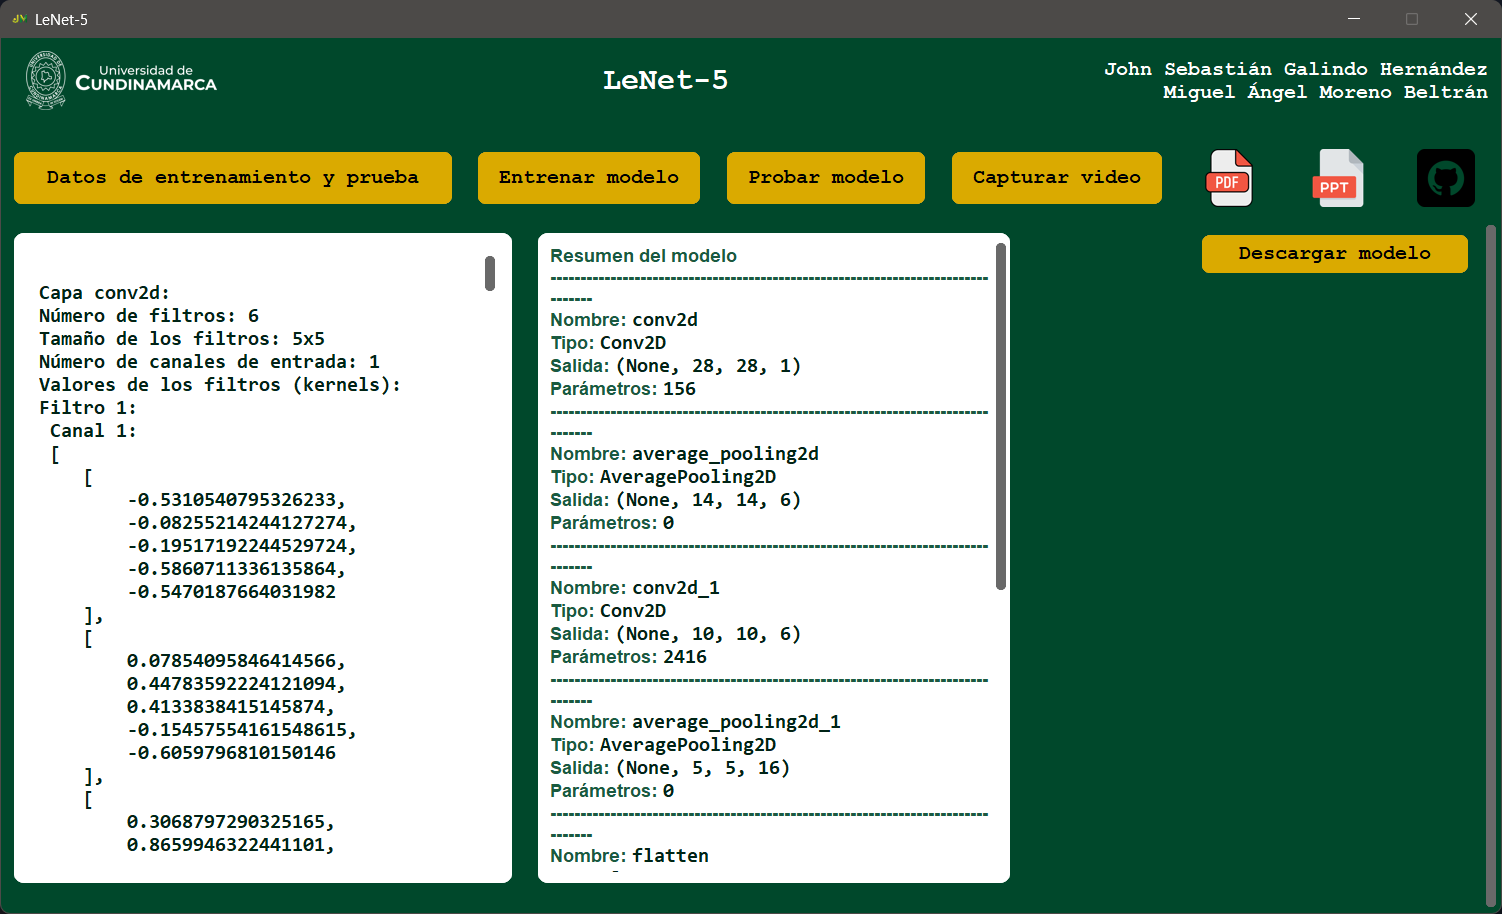
\includegraphics[width=\linewidth]{src/figures/datos_entrenamiento.png}
        \caption{Entrenamiento de la Red}
        \label{fig:data_training}
    \end{figure}

    \item \textbf{Probar la Red:} El usuario puede probar la red neuronal LeNet 5 con la imagen que el 
    seleccione desde el explorador de archivos, la red carga la imagen y la procesa para adecuarla a la red
    redimensionando la imagen y convirtiendola a escala de grises, después de esto la red realiza la predicción
    y se muestra tanto la imagen procesada como la predicción y las probabilidades de cada clase.

    \begin{figure}[H]
        \centering
        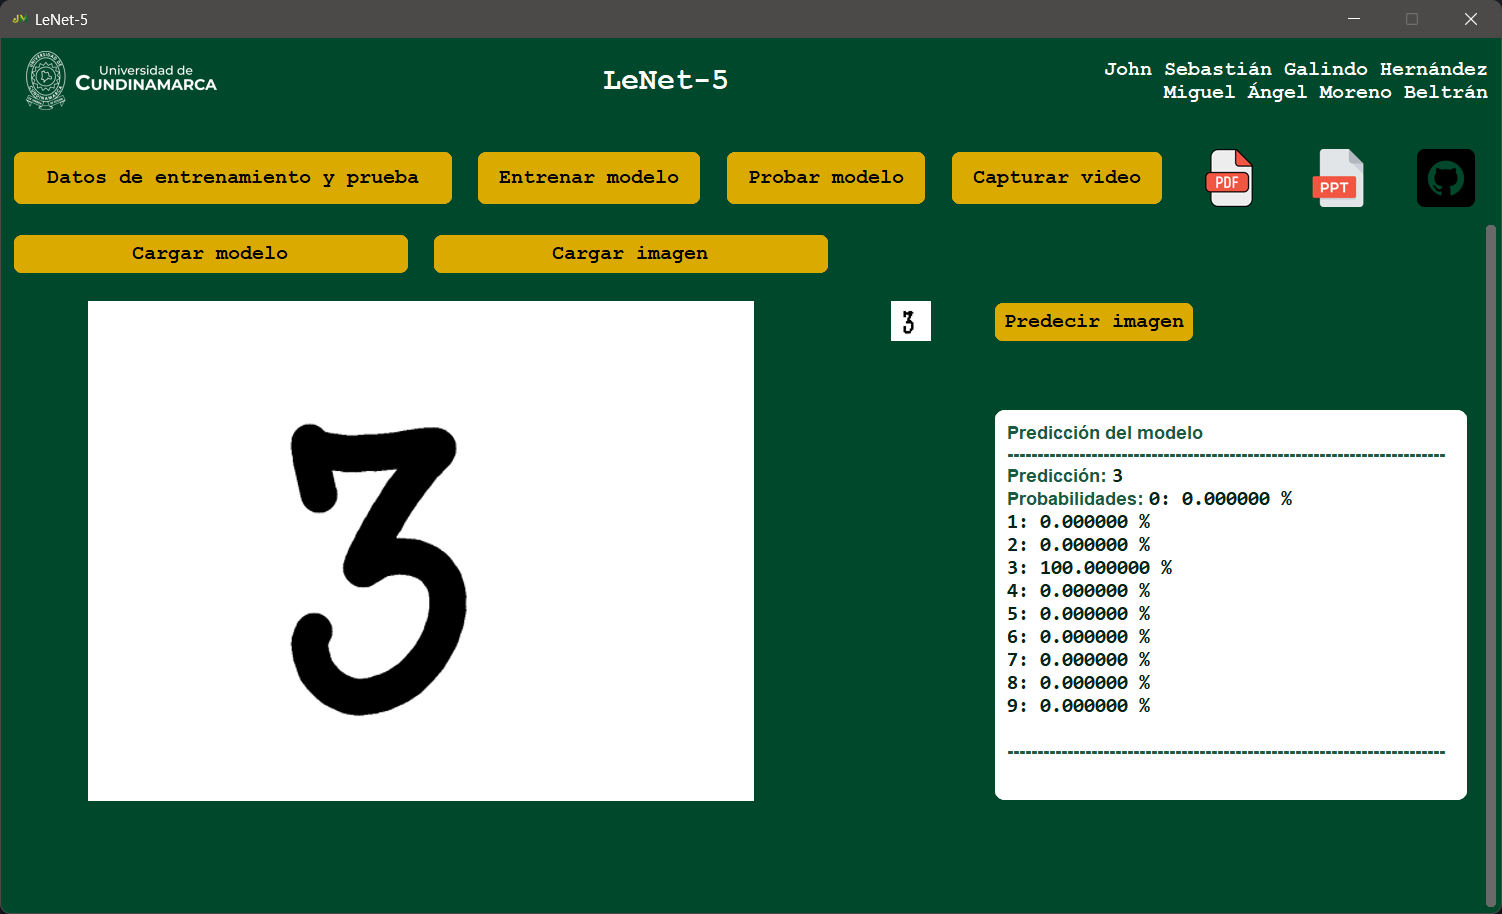
\includegraphics[width=\linewidth]{src/figures/prediccion_funcion.png}
        \caption{Sección de prueba de la Red}
        \label{fig:Test}
    \end{figure}

    \item \textbf{Capturar video:} El usuario puede capturar un video con la cámara de su computadora, la
    cámara que tenga conectada o la camara por IP, ya que esta se especifica mediante un texto ingresado en la GUI.
    una vez se hace conexion con la camara especificada se puede capturar el video y la red realiza la predicción
    de los números que se encuentren en el en tiempo real.

    \begin{figure}[H]
        \centering
        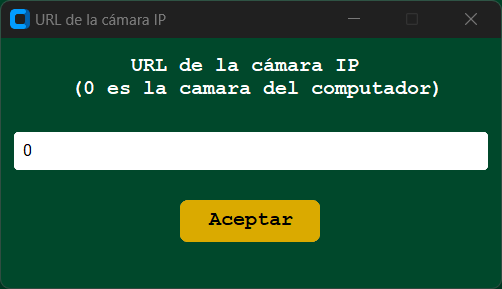
\includegraphics[width=\linewidth]{src/figures/url_camera.png}
        \caption{Sección de captura de Video}
        \label{fig:url_camera}
    \end{figure}

    \begin{figure}[H]
        \centering
        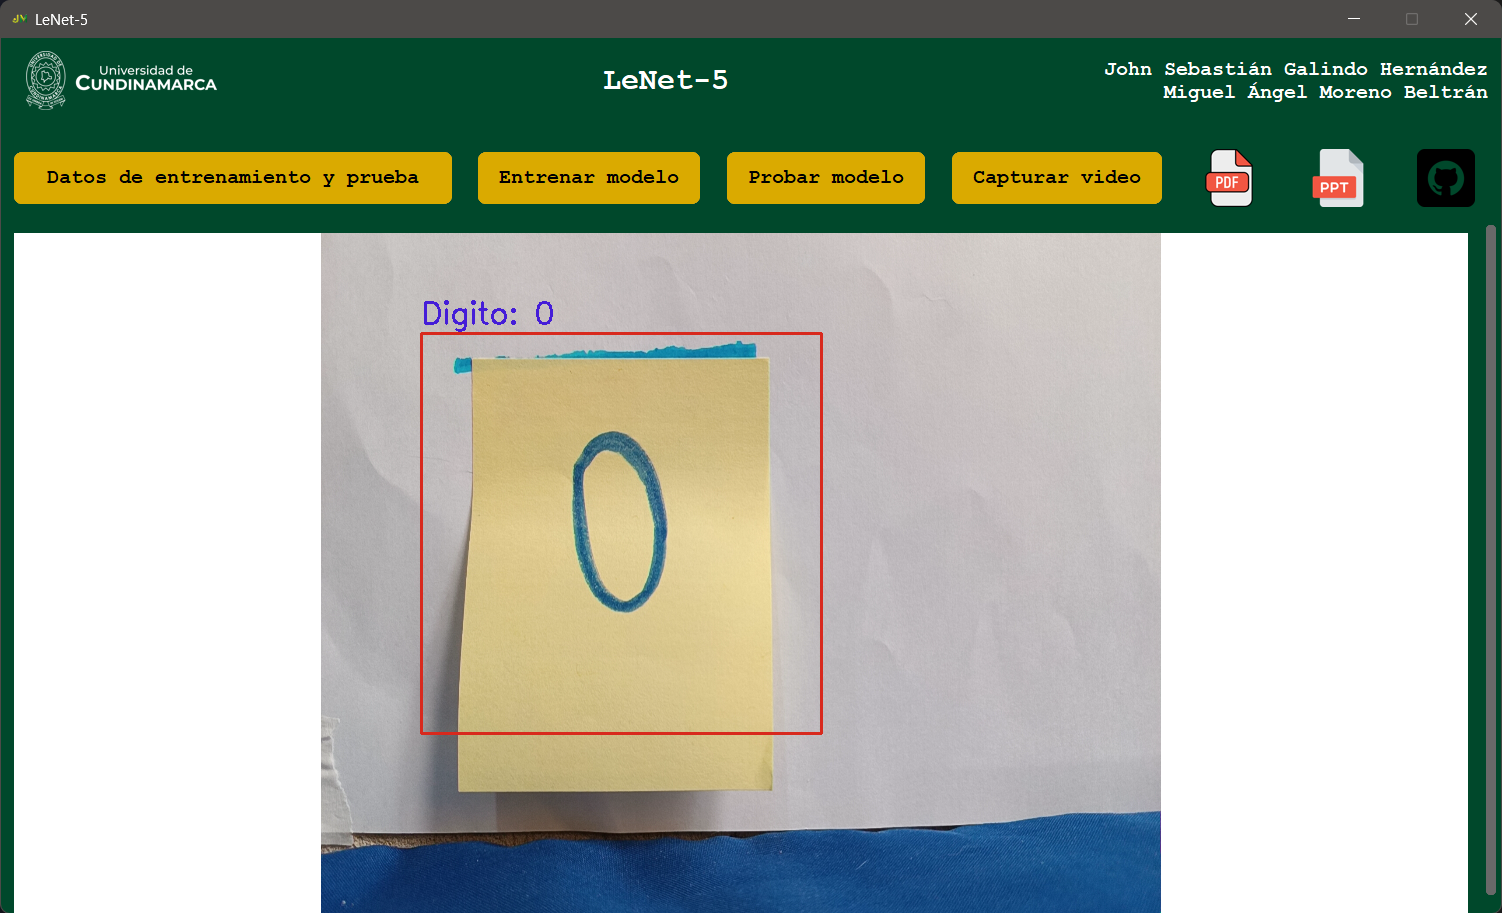
\includegraphics[width=\linewidth]{src/figures/real_test_image_0.png}
        \caption{Captura de Video}
        \label{fig:VideoCapture}
    \end{figure}
\end{itemize}

\subsection{Resultados del entrenamiento de la Red LeNet 5}
Para el entrenamiento de la red LeNet 5 se utilizo la base de datos de MNIST y SVHN, en ambos casos se
utilizó el optimizador adam y la función de activación ReLU para las capas ocultas, después de que 
se realizó el entrenamiento se obtuvieron los siguientes resultados:

\begin{figure}[htbp]
    \centering
    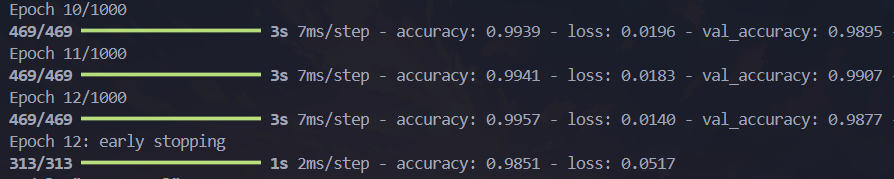
\includegraphics[width=1.1\linewidth]{src/figures/mnist_training.png}
    \caption{Resultados del entrenamiento con MNIST}
    \label{fig:MNISTResults}
\end{figure}

\begin{figure}[htbp]
    \centering
    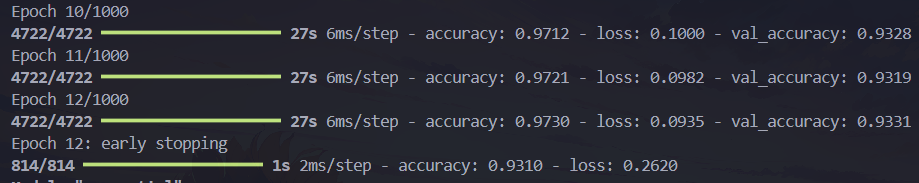
\includegraphics[width=1.1\linewidth]{src/figures/lenet_training.png}
    \caption{Resultados del entrenamiento con SVHN}
    \label{fig:SVHNResults}
\end{figure}

Como se puede comprobar, los resultados obtenidos en el entrenamiento de la red LeNet 5 con la base de datos
MNIST y SVHN son muy buenos, ya que en ambos casos se obtuvo una precisión por encima del 90\% en el conjunto
sin embargo al tener menos datos MNIST y al necesitar que las imagenes esten con la escala de grises invertida
se obtiene una menor tasa de acierto en la predicción de los números que no estén lo suficientemente contrastados
con el fondo. Es por este motivo, que se recomienda el uso de la base de datos SVHN para el entrenamiento de la red
ya que se han realizado pruebas con la base de datos y se ha obtenido una precisión muy alta con imagenes con un 
ruido muy alto.

Por otra parte, se realiza la comparación entre el entrenamiento dado en la figura \ref{fig:SVHNResults} y
los mismos datos con las funciones de activación (Tangente Híperbolica) y el optimizador de gradiente descendiente los
cuales se usaban originalmente en la red LeNet 5, los resultados obtenidos para la prueba original son los siguientes:

\begin{figure}[htbp]
    \centering
    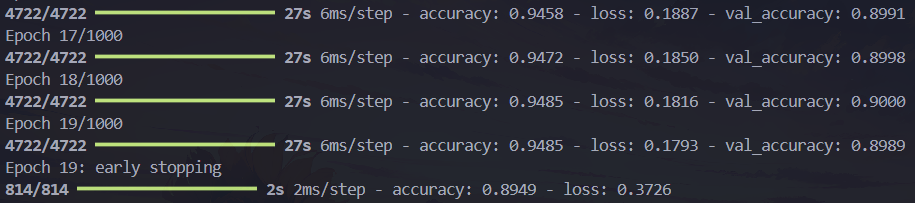
\includegraphics[width=\linewidth]{src/figures/original_info_training.png}
    \caption{Resultados del entrenamiento con SVHN}
    \label{fig:SVHNResultsOriginal}
\end{figure}

Como se puede observar, los resultados obtenidos con la función de activación ReLU y el optimizador Adam son
mejores que los obtenidos con la función de activación Tangente Híperbolica y el optimizador de gradiente descendiente,
ya que no solo alcanza una precisión mayor, sino que también el tiempo de entrenamiento es menor, para el entrenamiento
con los hiperparametros orginales el tiempo total fue de 9 minutos y 30 segundos logrando una precisión en el conjunto de
prueba de 89.5\% mientras que con los nuevos hiperparametros (ReLU y Adam) el tiempo total fue de 5 minutos y 30 segundos 
logrando una precisión en el conjunto de prueba de 93.1\%.

\subsection{Resultados de la Predicción de la Red LeNet 5}

Para la predicción de la red LeNet 5 se utilizo la base de datos de MNIST y SVHN, en ambos casos se tuvieron
algunos errores cuando los datos no estaban tenian muchas irregularidades o cuando su posicion no era la adecuada,
aún asi, con los datos de MNIST se obtuvo un grande error con al probar con imagenes de numeros que tienen estilos 
de caligrafia. Por otro lado, con la base de datos SVHN se obtuvieron resultados muy buenos, tanto para caligrafias
de computadora como para datos escritos a mano e incluso para imagenes de numeros en pinturas o con texturas muy
ruidosas.

Uno de los ejemplos de un resultado presentado trabajando con el modelo entrenado con la base de datos SVHN es el
siguiente:

\begin{figure}[htbp]
    \centering
    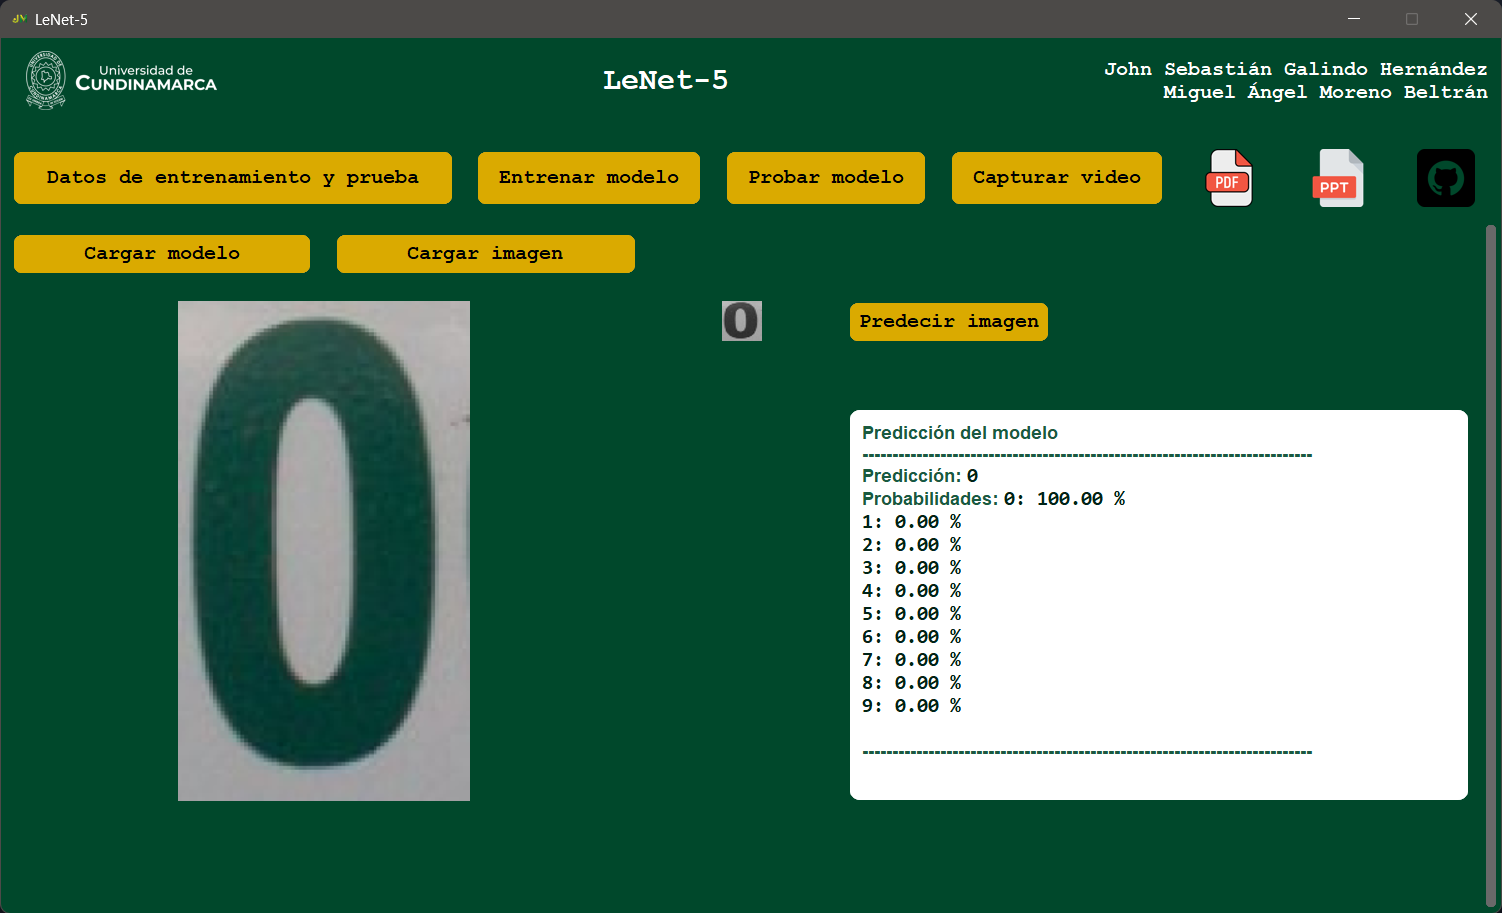
\includegraphics[width=\linewidth]{src/figures/pic_test_image_0.png}
    \caption{Predicción de la Red LeNet 5 para el número 0}
    \label{fig:Prediction_pic_0}
\end{figure}

\begin{figure}[htbp]
    \centering
    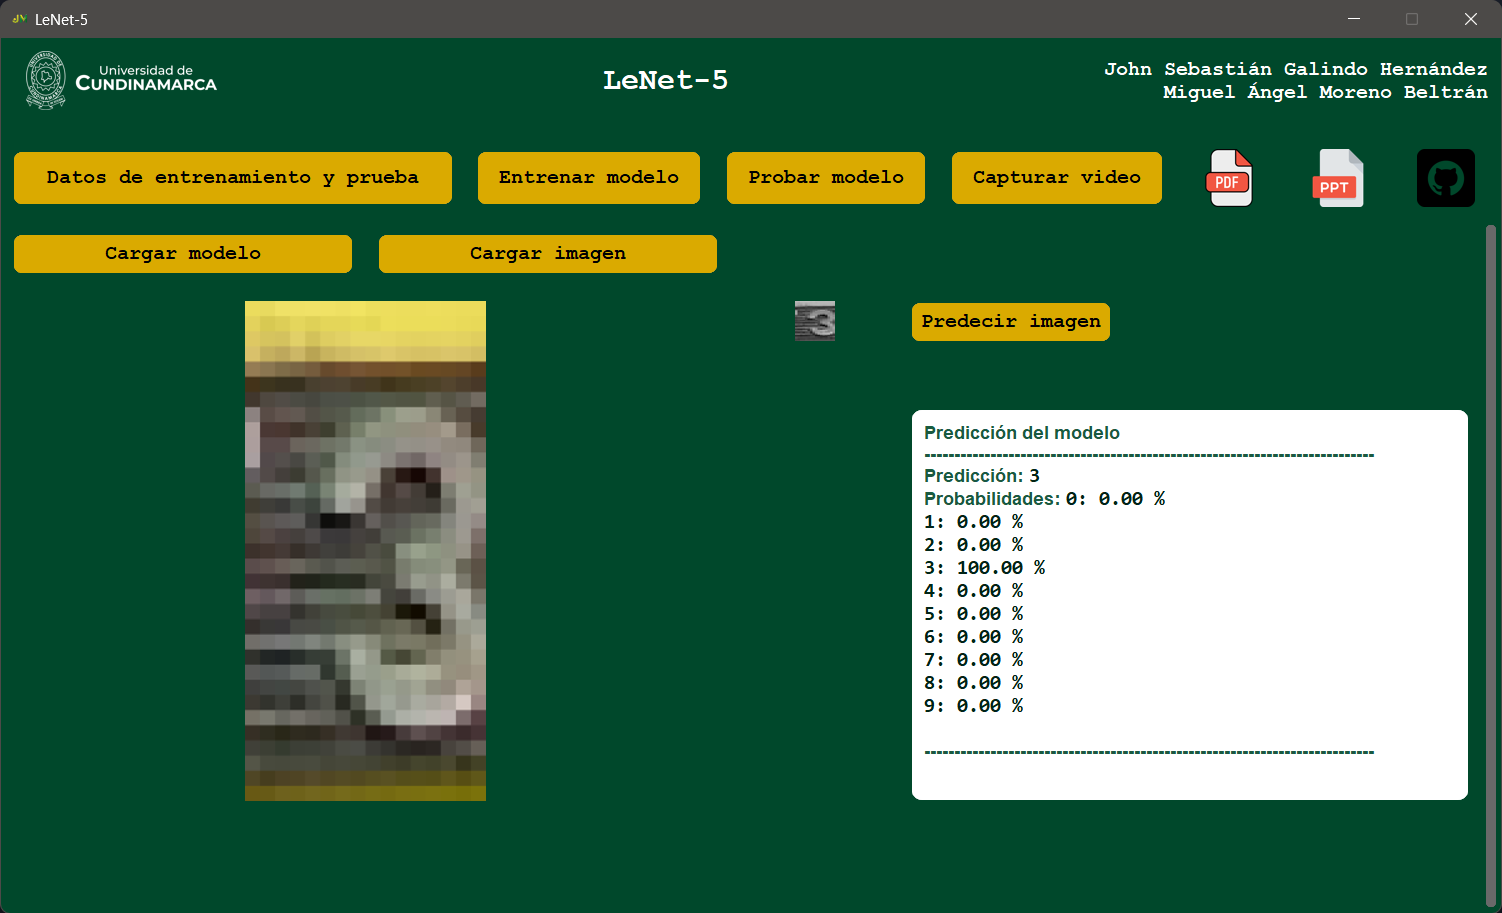
\includegraphics[width=1.05\linewidth]{src/figures/pic_test_image_3.png}
    \caption{Predicción de la Red LeNet 5 para el número 3 con baja resolución}
    \label{fig:Prediction_pic_1}
\end{figure}

Aún cuando hay resultados buenos, el modelo no es perfecto y se puede mejorar, por ejemplo, en la 
siguiente predicción se puede observar que el modelo no es capaz de predecir correctamente el número y 
termina distribuyendo la probabilidad entre varios números lo cual no es habitual en la red LeNet 5.

\begin{figure}[htbp]
    \centering
    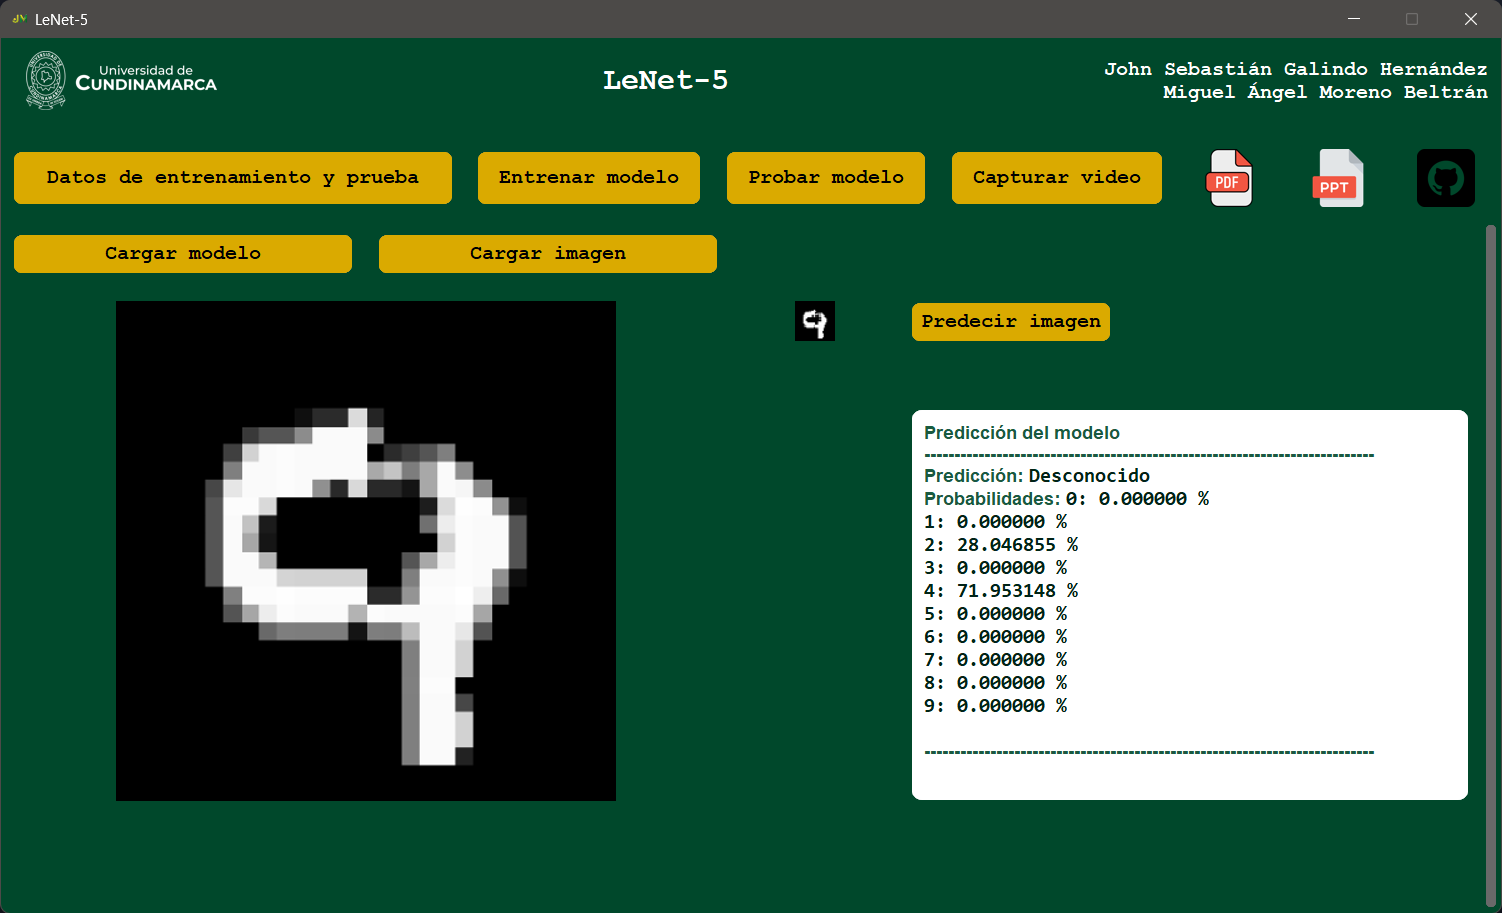
\includegraphics[width=1.05\linewidth]{src/figures/pic_test_image_prob.png}
    \caption{Predicción de la Red LeNet 5 para el número 9}
    \label{fig:Prediction_pic_2}
\end{figure}

todas las imagenes de prueba fueron obtenidas del conjunto de datos Numerical Images encontrado en 
la pagina web de \textbf{Kaggle} \cite{kaggle_data}.

\subsection{Resultados de la Captura de Video}

Para la captura de video se utilizo la cámara de un celular conectado mediante IP con una resolución de 
1080p, en la captura de video se obtuvieron resultados muy buenos pero que eran muy susceptibles a la
posicion del número en el recuadro de información, ya que si el número no estaba centrado o si estaba
muy inclinado la red no era capaz de predecir correctamente el número, sin embargo, los resultados 
en general fueron muy buenos y se obtuvo un resultado correcto en la gran mayoría de los casos.
A continuación se presentan una serie de pruebas realizadas para los numeros desde el 0 hasta el 9.

\begin{figure}[H]
    \centering
    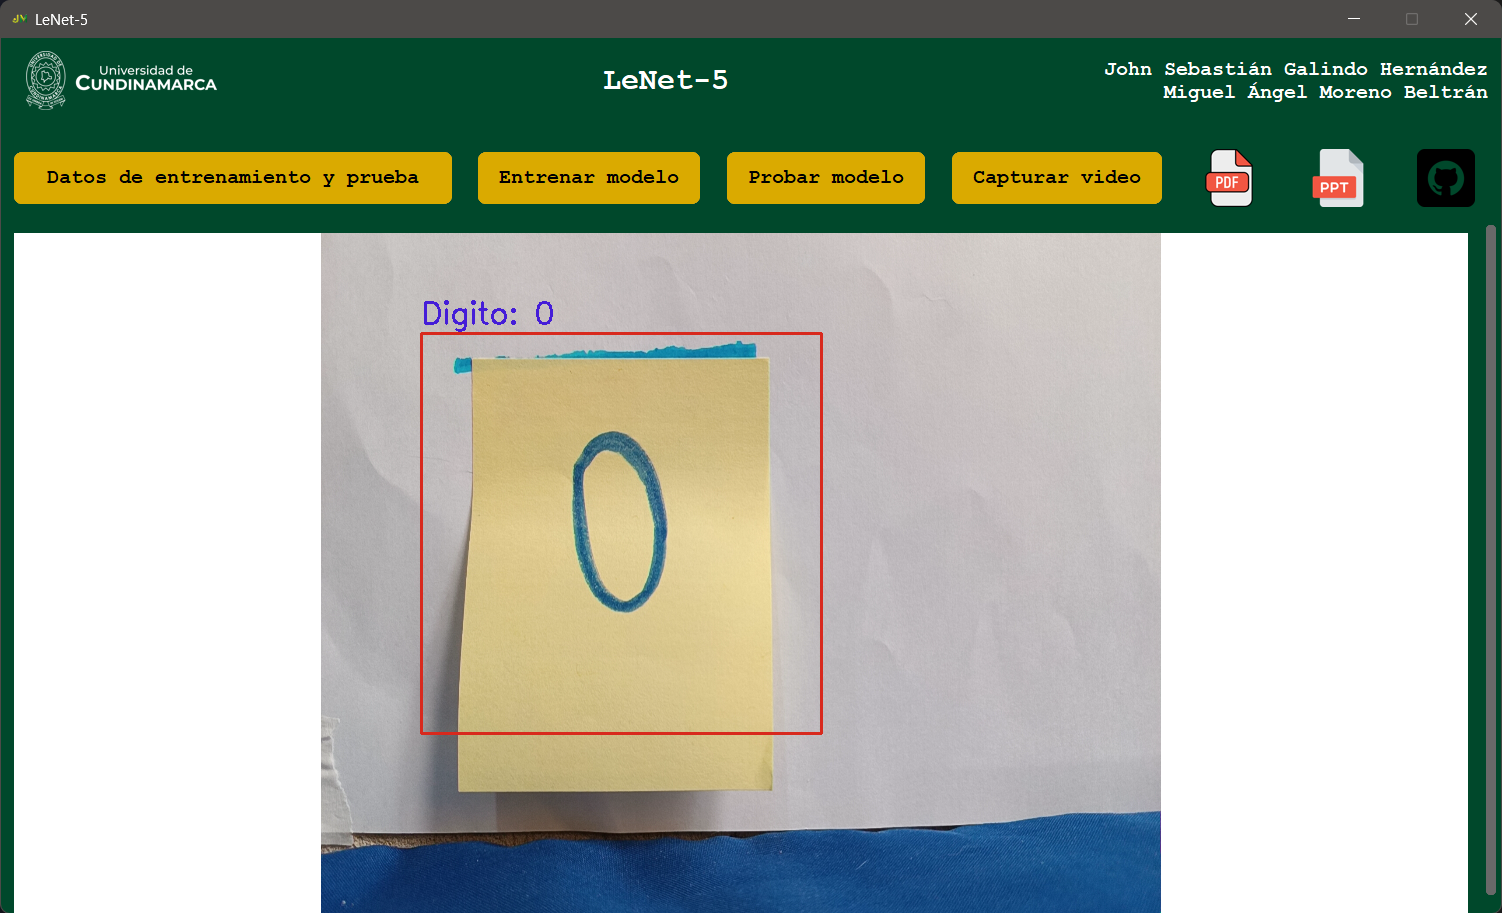
\includegraphics[width=\linewidth]{src/figures/real_test_image_0.png}
    \caption{Predicción en tiempo real de la Red LeNet 5 para el número 0}
    \label{fig:RealTest_0}
\end{figure}

\begin{figure}[H]
    \centering
    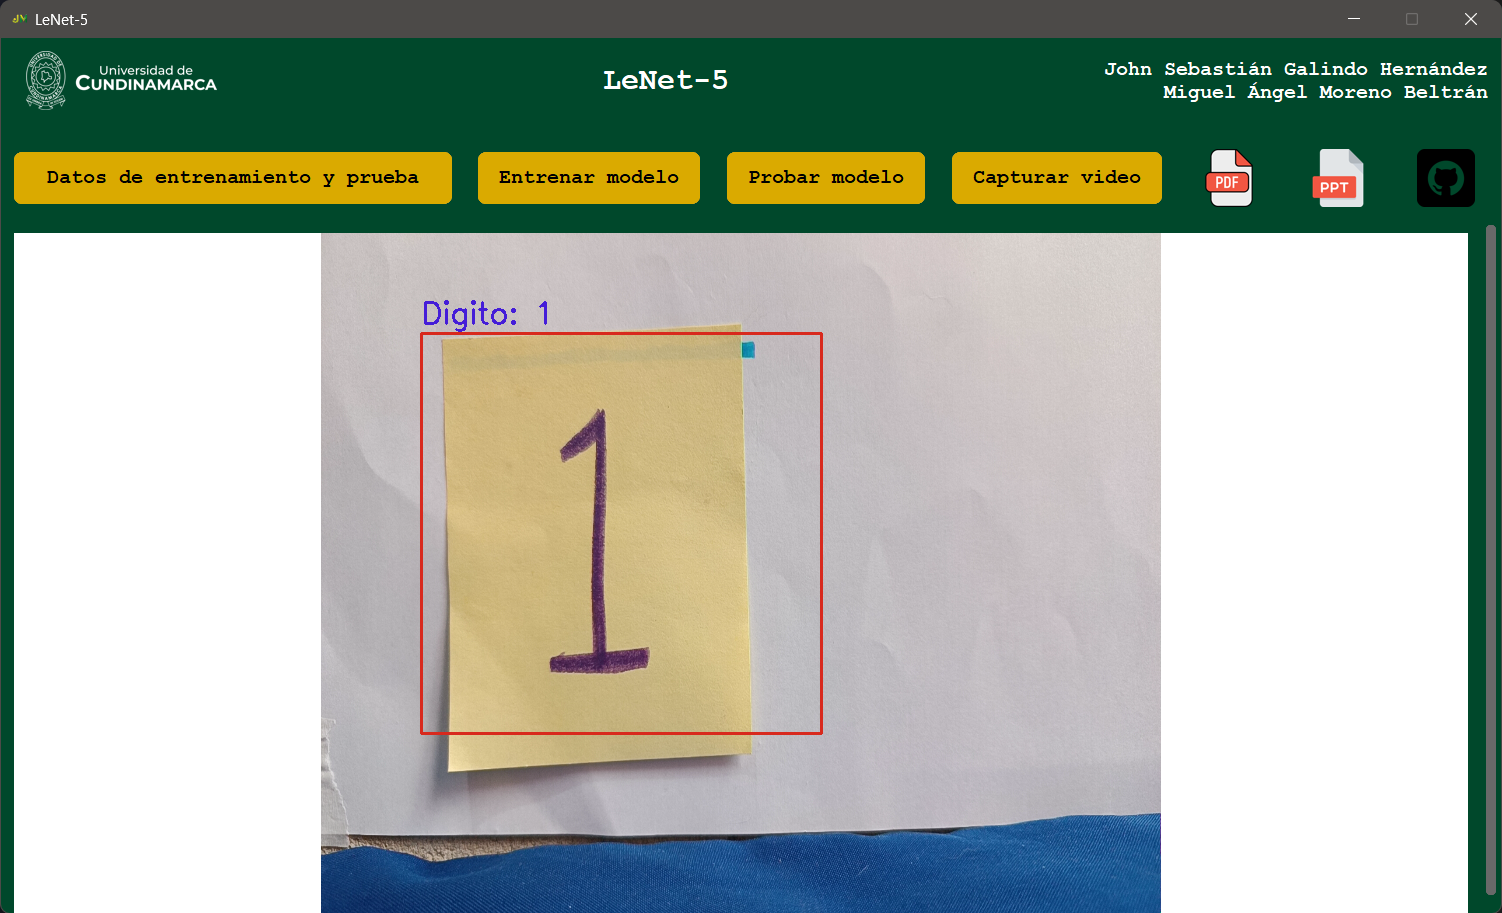
\includegraphics[width=\linewidth]{src/figures/real_test_image_1.png}
    \caption{Predicción en tiempo real de la Red LeNet 5 para el número 1}
    \label{fig:RealTest_1}
\end{figure}

\begin{figure}[H]
    \centering
    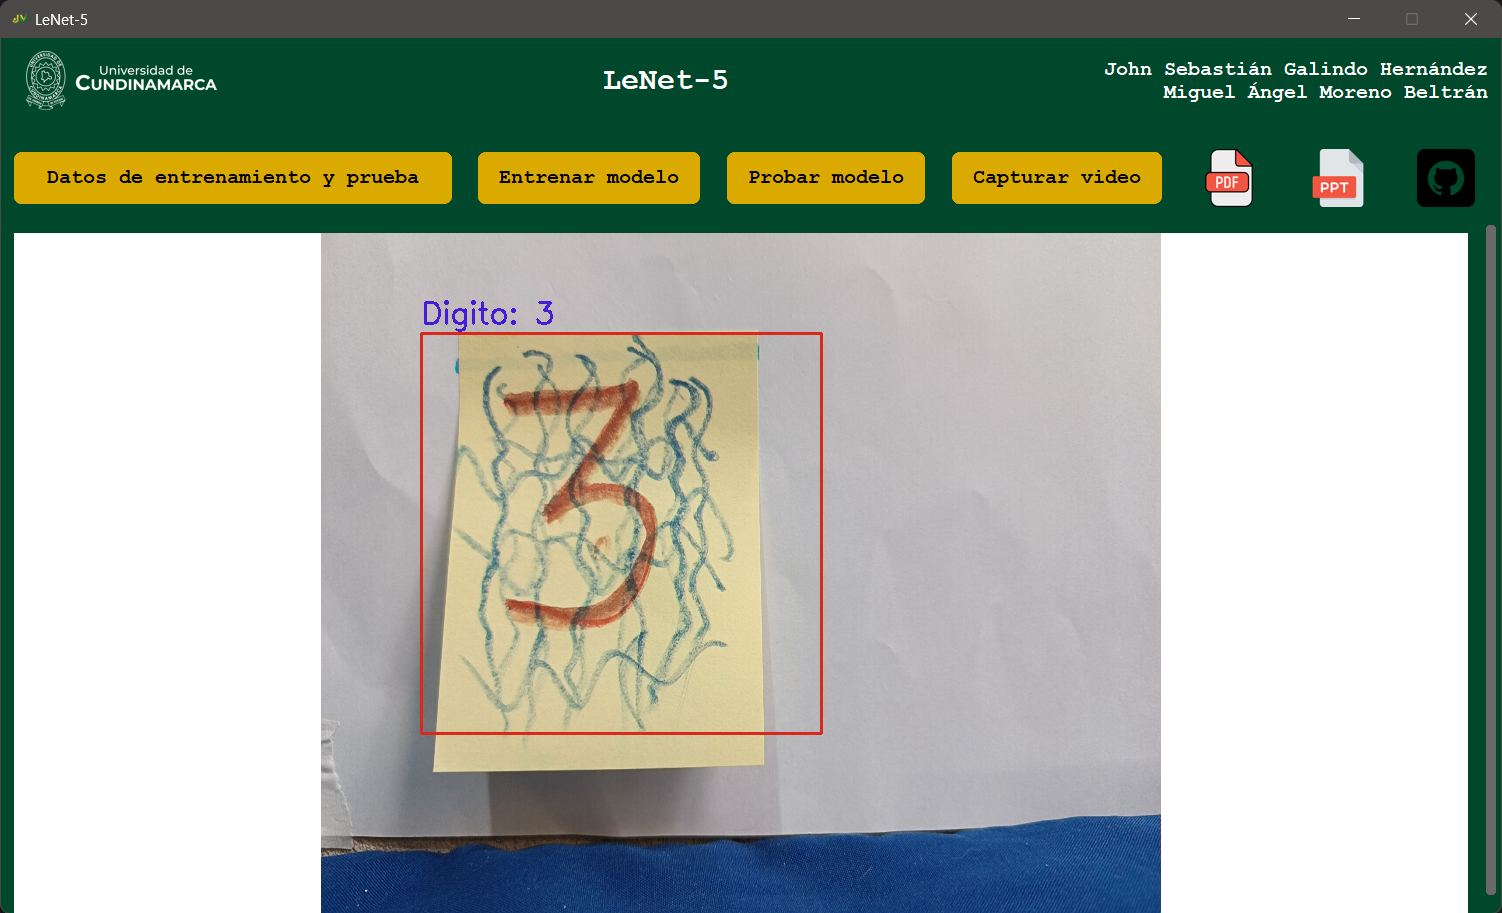
\includegraphics[width=\linewidth]{src/figures/real_test_image_3.png}
    \caption{Predicción en tiempo real de la Red LeNet 5 para el número 3}
    \label{fig:RealTest_3}
\end{figure}

\begin{figure}[H]
    \centering
    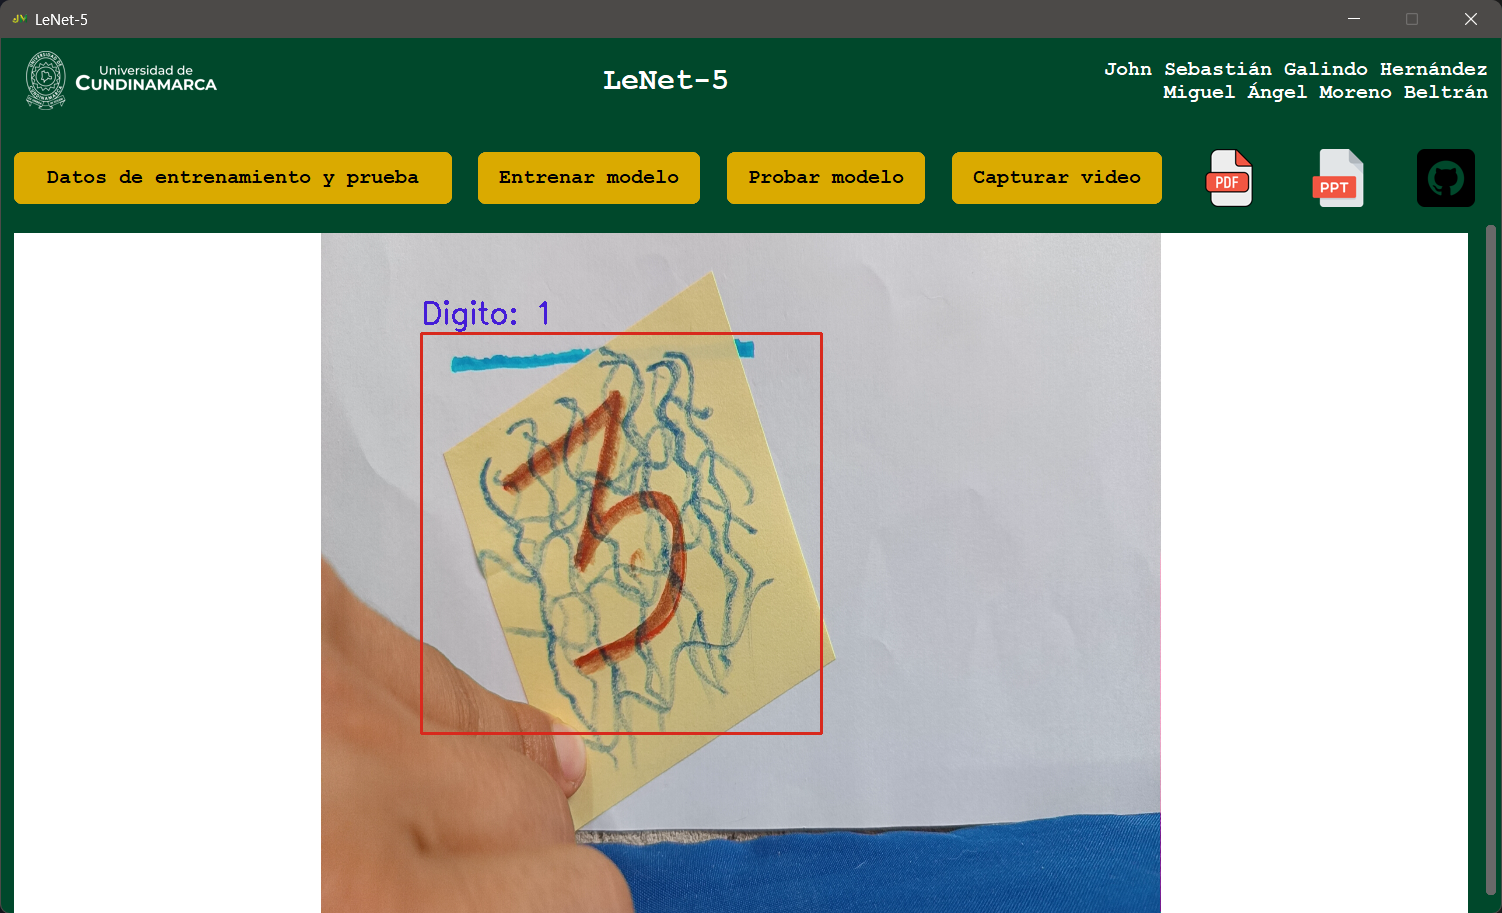
\includegraphics[width=\linewidth]{src/figures/real_test_image_3-2.png}
    \caption{Predicción en tiempo real de la Red LeNet 5 para el número 3 inclinado}
    \label{fig:RealTest_3_2}
\end{figure}

\begin{figure}[H]
    \centering
    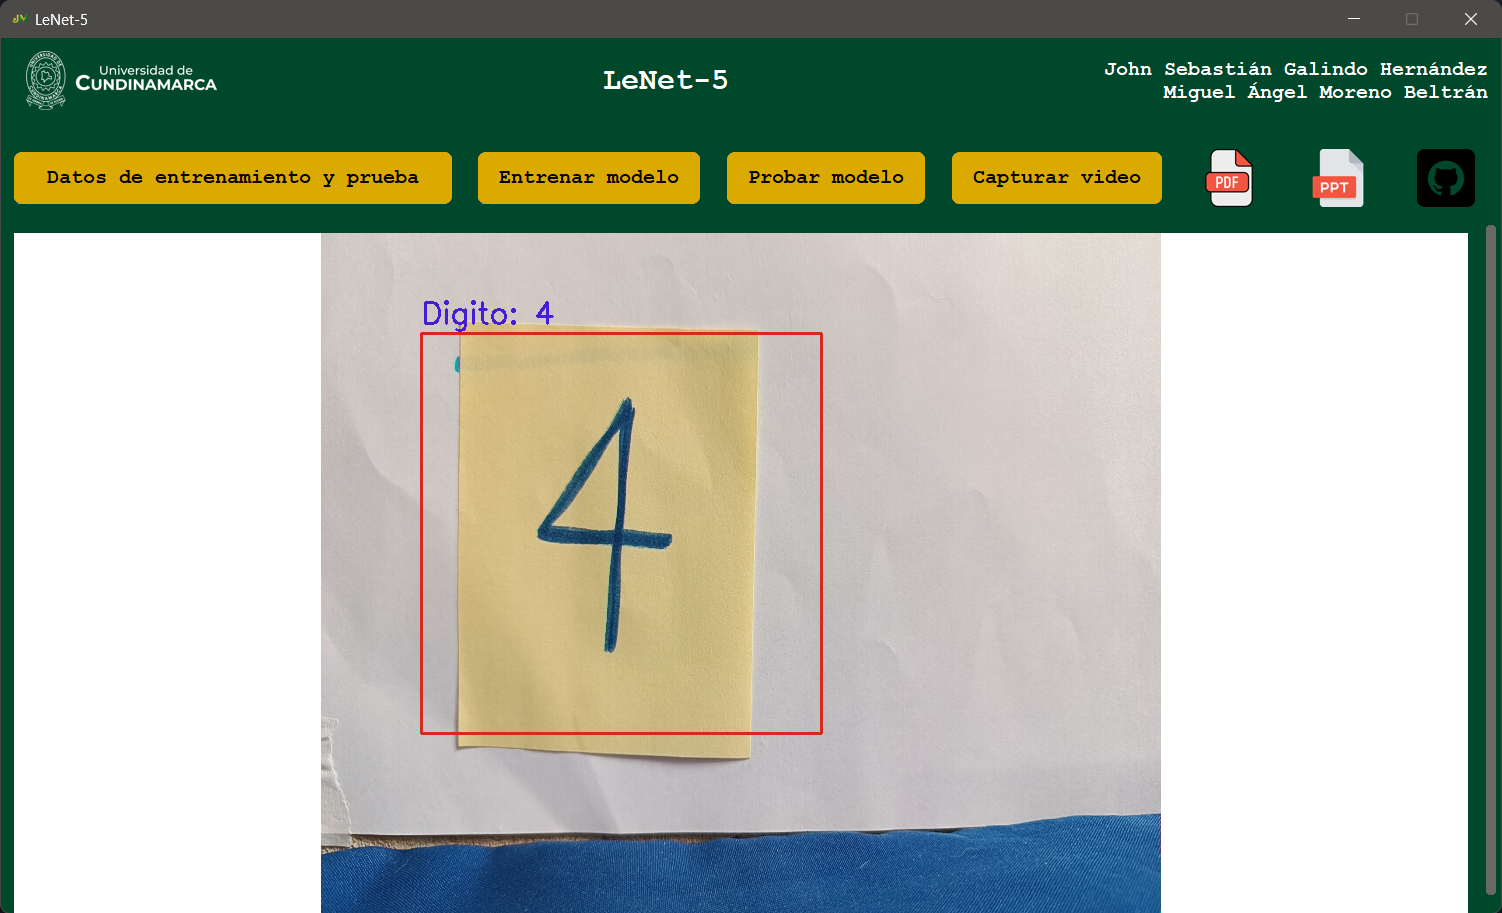
\includegraphics[width=\linewidth]{src/figures/real_test_image_4.png}
    \caption{Predicción en tiempo real de la Red LeNet 5 para el número 4}
    \label{fig:RealTest_4}
\end{figure}

\begin{figure}[H]
    \centering
    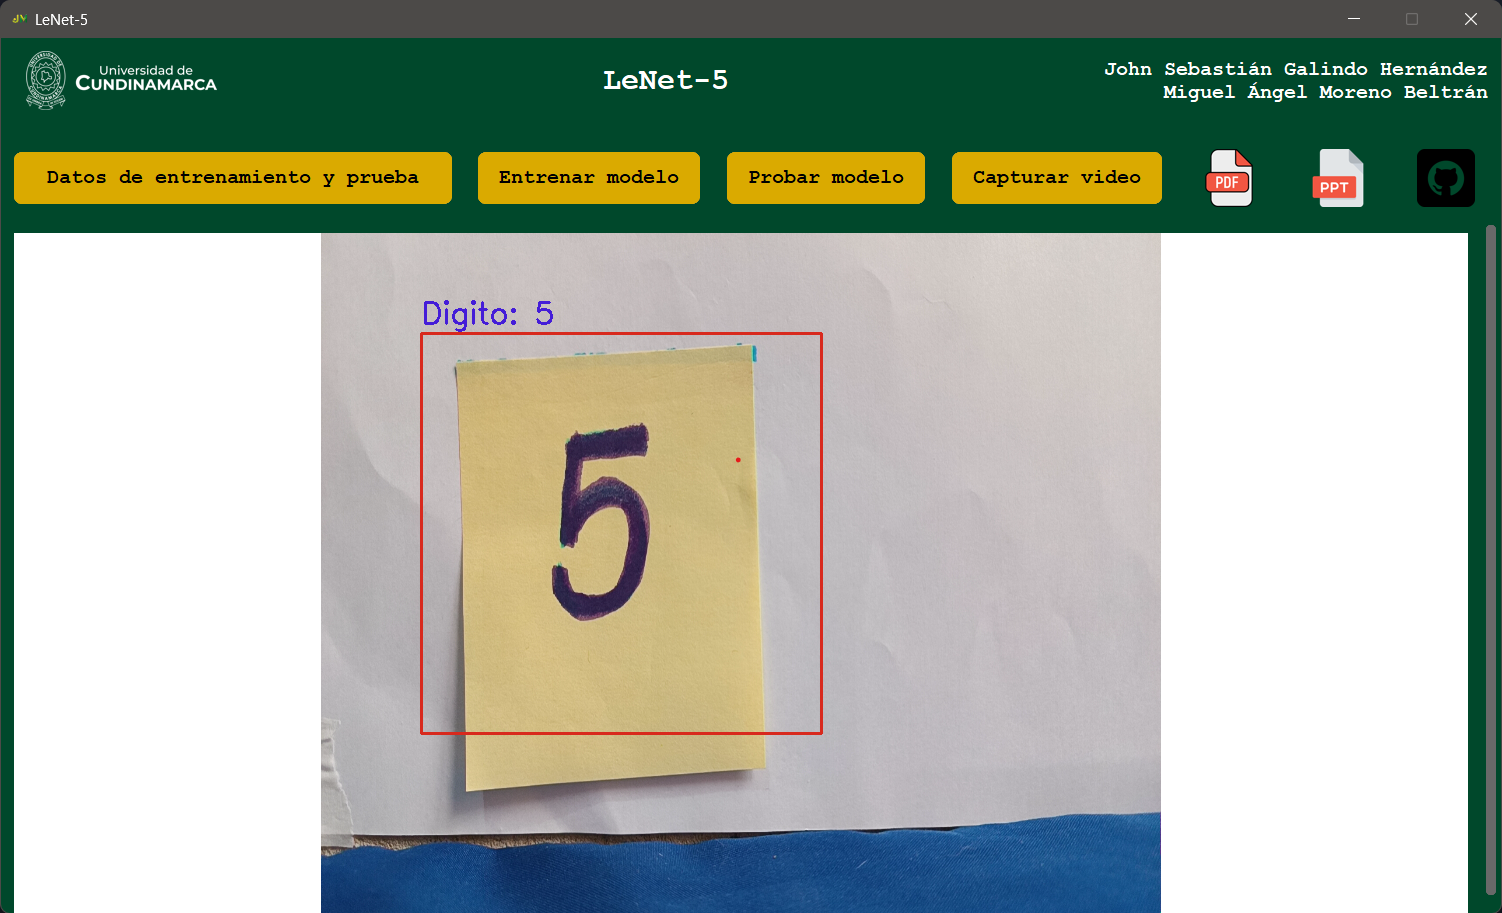
\includegraphics[width=\linewidth]{src/figures/real_test_image_5.png}
    \caption{Predicción en tiempo real de la Red LeNet 5 para el número 5}
    \label{fig:RealTest_5}
\end{figure}

\begin{figure}[H]
    \centering
    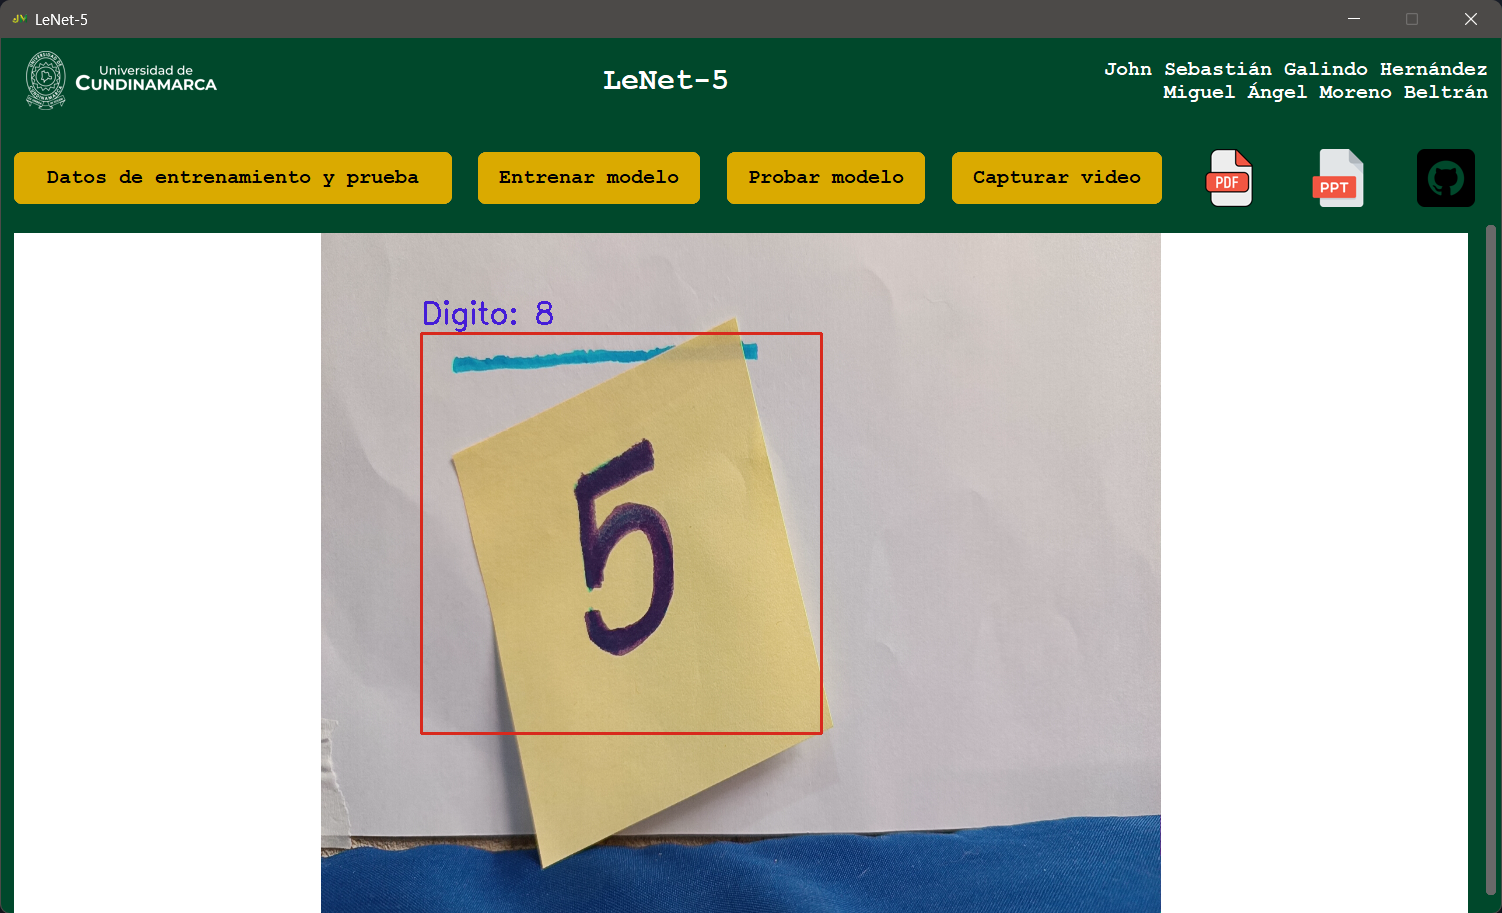
\includegraphics[width=\linewidth]{src/figures/real_test_image_5-2.png}
    \caption{Predicción en tiempo real de la Red LeNet 5 para el número 5 inclinado}
    \label{fig:RealTest_5_2}
\end{figure}

\begin{figure}[H]
    \centering
    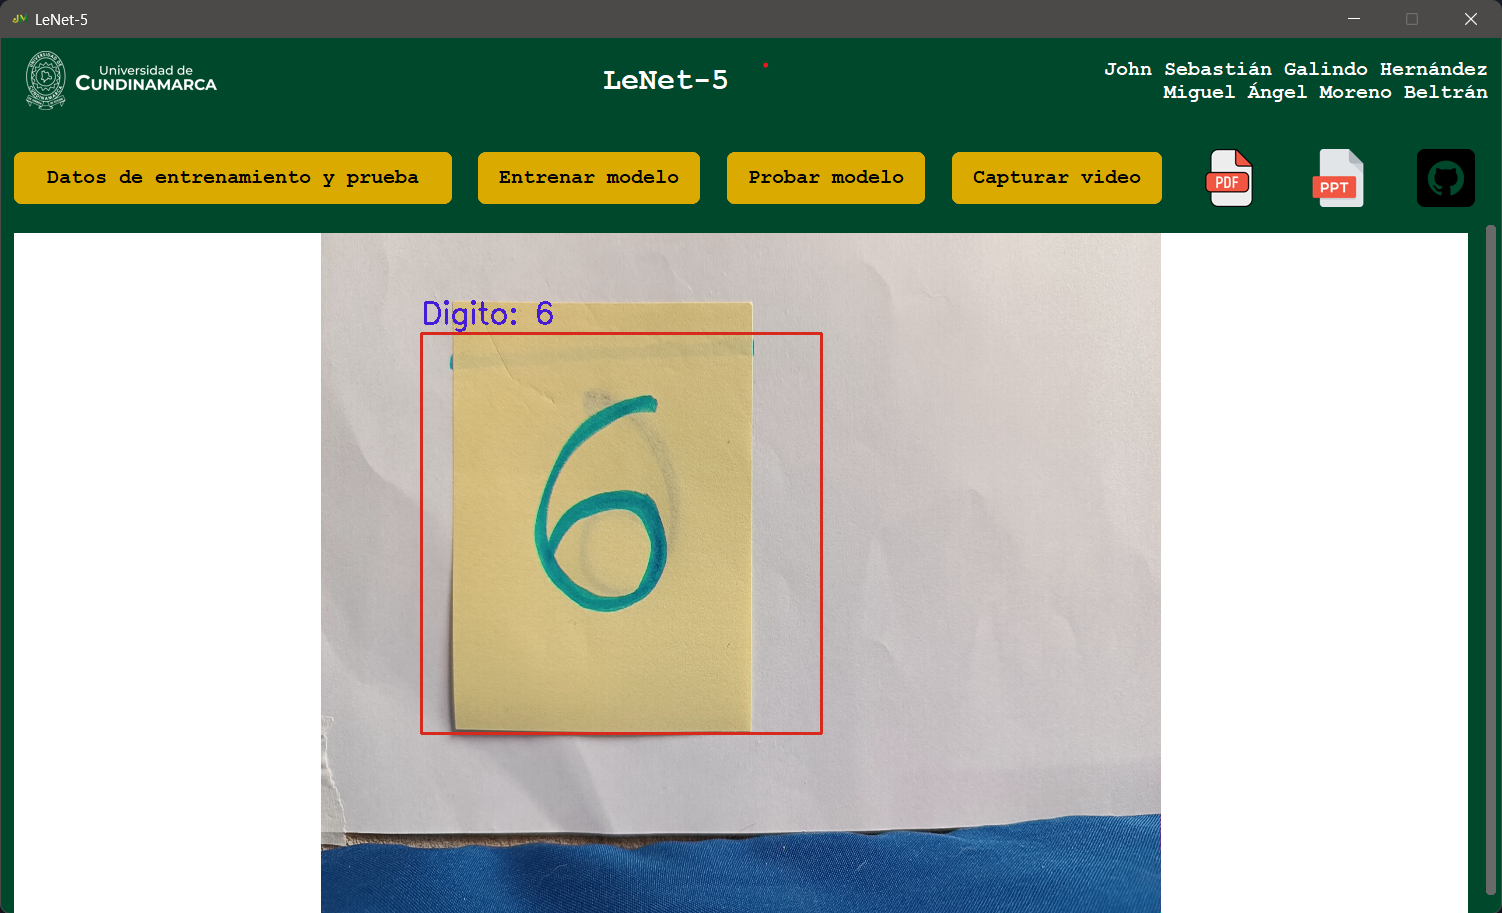
\includegraphics[width=\linewidth]{src/figures/real_test_image_6.png}
    \caption{Predicción en tiempo real de la Red LeNet 5 para el número 6}
    \label{fig:RealTest_6}
\end{figure}

\begin{figure}[H]
    \centering
    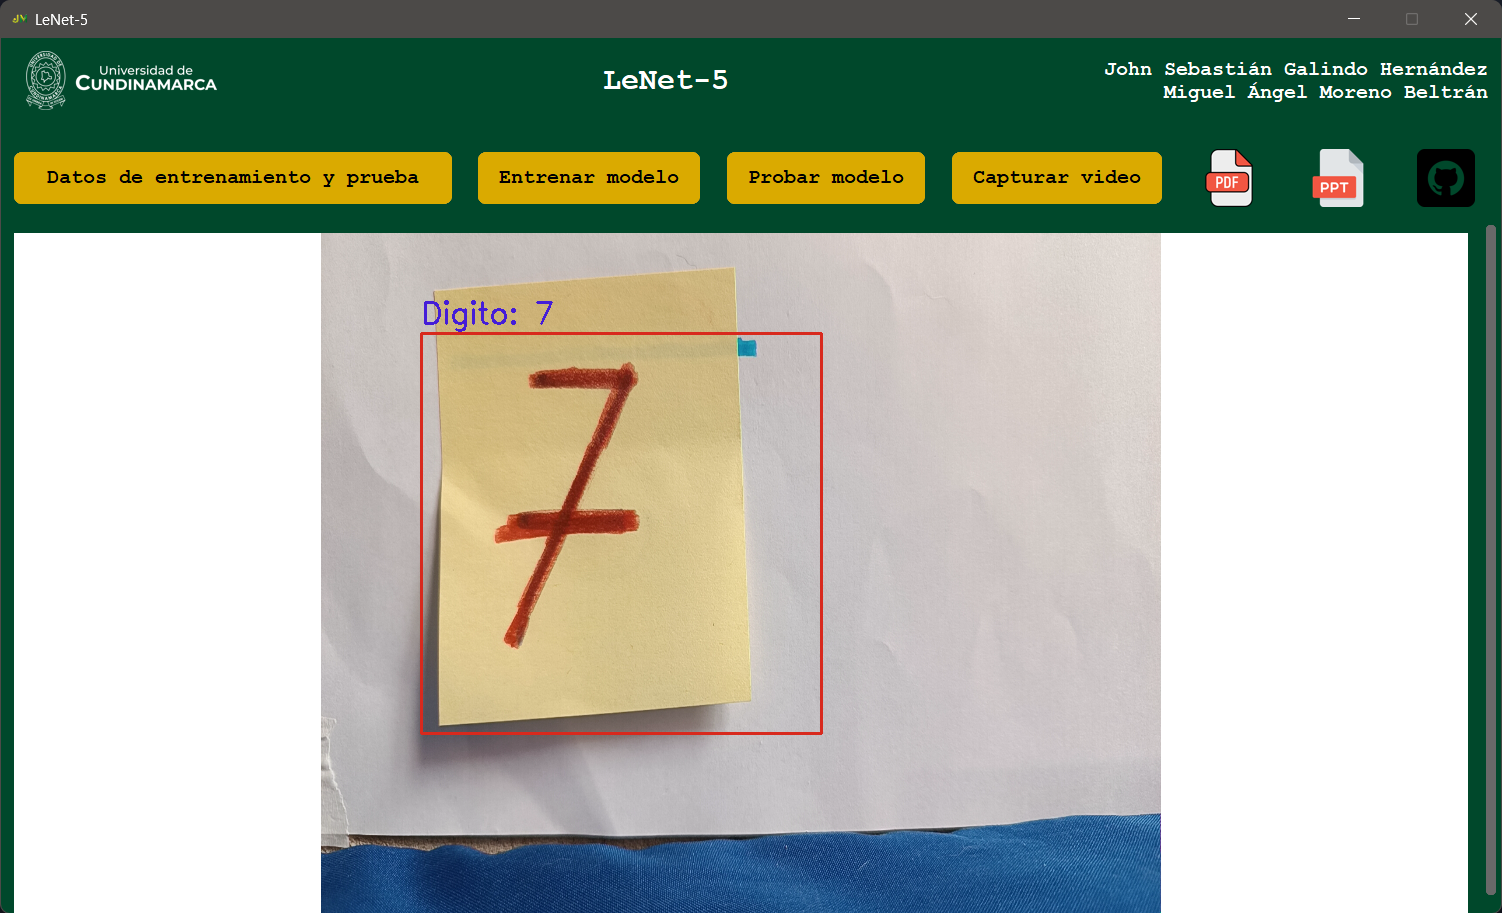
\includegraphics[width=\linewidth]{src/figures/real_test_image_7.png}
    \caption{Predicción en tiempo real de la Red LeNet 5 para el número 7}
    \label{fig:RealTest_7}
\end{figure}

\begin{figure}[H]
    \centering
    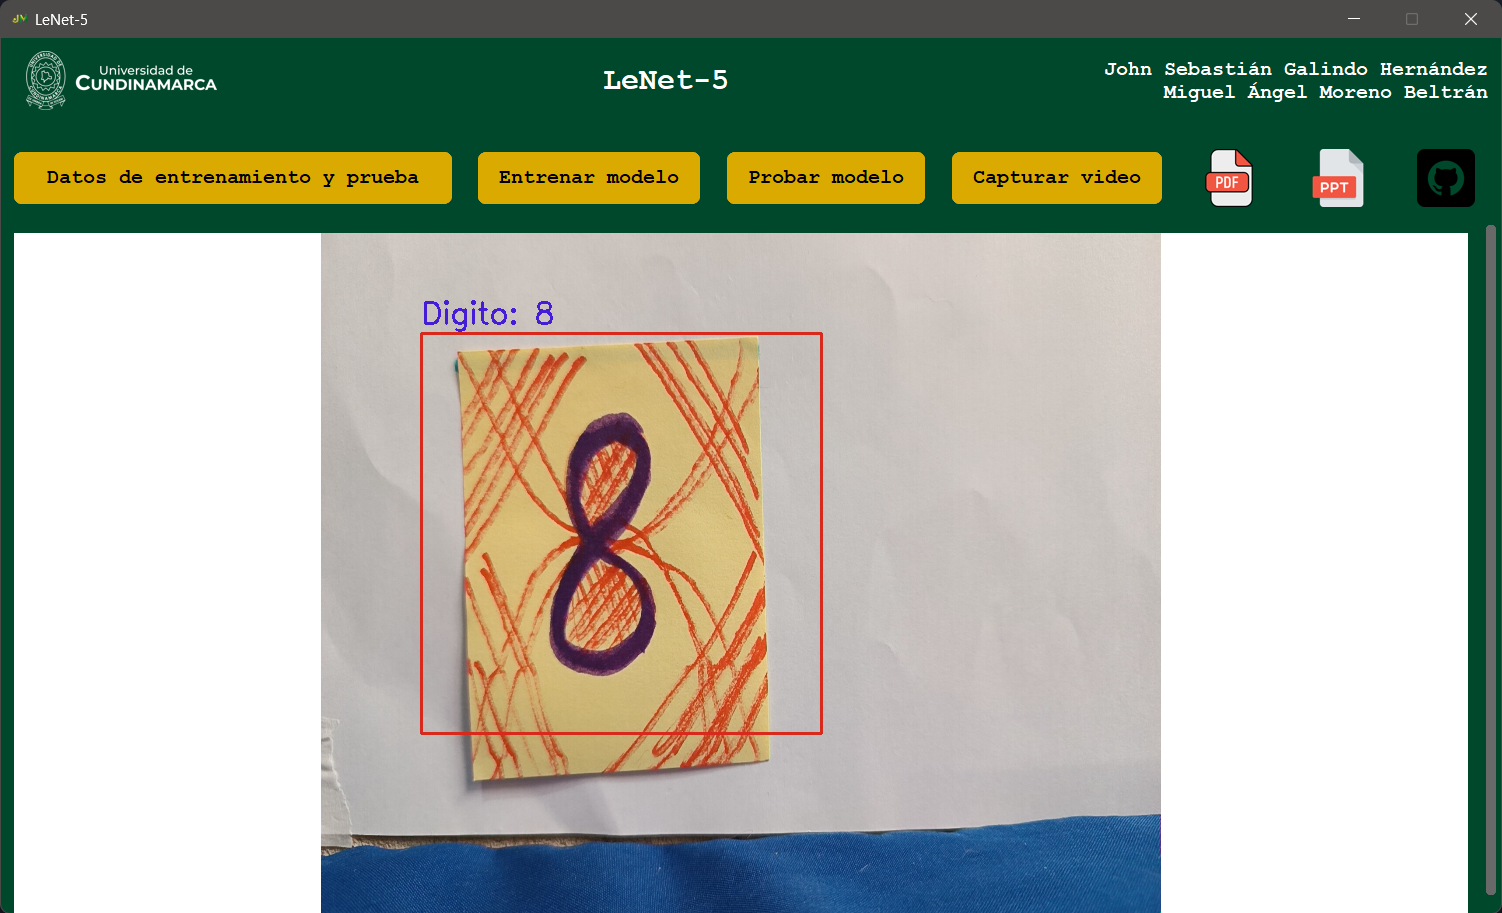
\includegraphics[width=\linewidth]{src/figures/real_test_image_8.png}
    \caption{Predicción en tiempo real de la Red LeNet 5 para el número 8}
    \label{fig:RealTest_8}
\end{figure}

\begin{figure}[H]
    \centering
    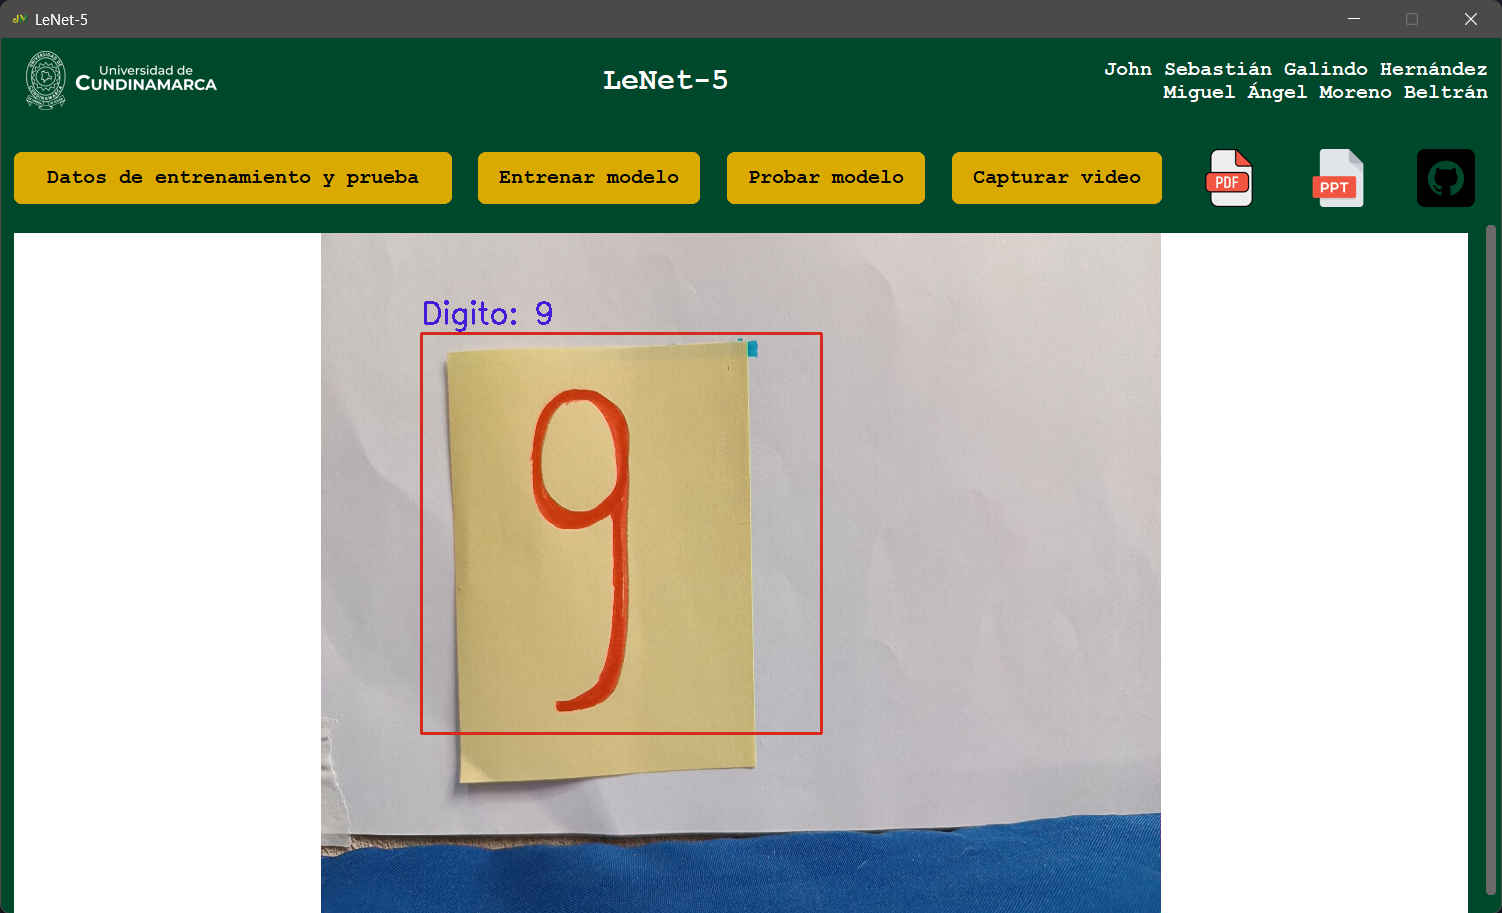
\includegraphics[width=\linewidth]{src/figures/real_test_image_9.png}
    \caption{Predicción en tiempo real de la Red LeNet 5 para el número 9}
    \label{fig:RealTest_9}
\end{figure}

Como se puede ver en las imagenes, se implemento una region de interés (ROI) para que la red solo procese
la parte de la imagen que contiene el número, esto se hizo para mejorar la predicción de la red y para que
la red no se vea afectada por el ruido de la imagen. Por otro lado, se corrobora que ni el ruido ni el color
del número afectan la predicción de la red, ya que se realizaron pruebas con números de diferentes colores y
con números con rayones y la red fue capaz de predecir correctamente el número en la gran mayoría de los casos; 
sin embargo, la red no es perfecta y en algunos casos no es capaz de predecir correctamente el número, sobre todo
cuando el número no esta centrado o cuando el número esta muy inclinado hacia alguno de sus lados, lo que demuestra
que los filtros de la red aprendieron a identificar patrones en base a la posición del número en la imagen, lo cual
cobra sentido al saber que debe diferenciar entre formas similares pero en diferente posicion como las del 6 y el 9.